\subsection{Convergence-based adaptation window}
\label{subsec:pers_convergence}

\paragraph{What we did.} The diagnostic above uses a fixed warm-up cutoff and shows no personalization effect. Here we fit an actual per-participant correction: for each participant, a per-horizon bias is estimated in closed form (mean forecast residual, no training loop) over the frozen model's adaptation-window anchors, then applied to held-out evaluation-window anchors. Rather than fixing the adaptation window at one value for everyone, we grow it in 6h increments up to a 48h ceiling and refit the correction independently at each step; a participant is marked \emph{converged} once the fitted correction stops moving (max change across horizons $<3$~mg/dL for 3 consecutive increments), and \texttt{convergence\_hours} records when that happens. All results use the frozen \texttt{aireadi\_stream\_mamba\_stateful\_5epoch} checkpoint, no weights updated. Phase boundaries were recomputed against the model's real train/val/test split (\texttt{adapt6h}, read as fixed ground truth) rather than the mismatched split originally used, leaving 132/221 test and 155/239 validation participants eligible for the 48h convention (287 total).

\paragraph{Experiment.} Tolerance and lookback were picked by inspecting raw correction trajectories on a 15-participant sample, including four participants pre-selected from an earlier diagnostic (one with sustained episodic residuals, two with high but evenly-spread variance, two whose correction had hurt evaluation MAE) to sanity-check the convergence signal against a known pattern before scaling up. We then ran the full 287-participant cohort, comparing three adaptation-window arms, fixed 24h, fixed 48h, and convergence-based, against the same held-out evaluation anchors, and cross-tabulated convergence status against MAE outcome rather than pooling them into one success rate.

\paragraph{Results.} 194/287 participants (67.6\%) converged within 48h; 93 (32.4\%) did not. Convergence\_hours clusters tightly in a 24--36h band (median 30h, p10 24h, p90 36h; Figure~\ref{fig:pers_conv_hours_hist}) and barely varies by subgroup, but the \emph{rate} of convergence drops with worse metabolic control (75\% to 54\% from lowest to highest HbA1c quartile; 74\% to 60\% by BMI quartile; insulin status has no effect).

\begin{figure}[t]
\centering
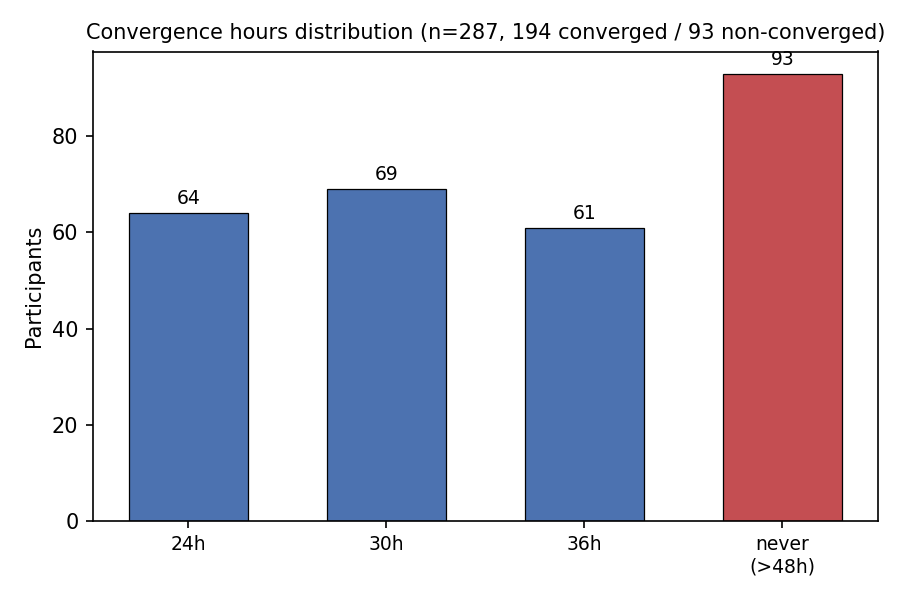
\includegraphics[width=0.62\linewidth]{figures/generated/personalization_convergence_hours_hist.png}
\caption{Convergence\_hours across the full cohort (n=287). Converged participants cluster in a 24--36h band; 93 never stabilize within 48h.}
\label{fig:pers_conv_hours_hist}
\end{figure}

Convergence does not imply the correction helps. Among the 194 converged participants, the correction still worsens MAE for the majority under every arm (58--61\% worsened; Figure~\ref{fig:pers_conv_mae_improvement}), and mean improvement is negative across the board (fixed 24h: $-0.191$~mg/dL; fixed 48h: $-0.168$; convergence-based: $-0.148$). The convergence-based window is the least-bad of the three, but only marginally, the more consequential result is that bias-only correction does not hold up at full-cohort scale regardless of window choice; the 15-participant pilot's 8/15 improvement rate was not representative.

\begin{figure}[t]
\centering
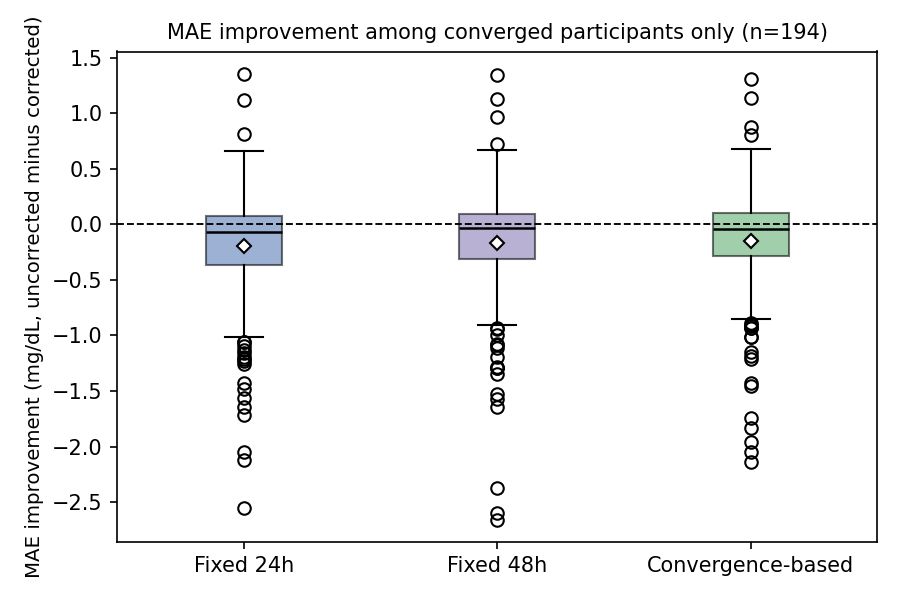
\includegraphics[width=0.62\linewidth]{figures/generated/personalization_mae_improvement_converged.png}
\caption{MAE improvement among the 194 converged participants, all three arms. Median and mean sit at or below zero everywhere; diamonds mark the mean.}
\label{fig:pers_conv_mae_improvement}
\end{figure}

Cross-tabulating convergence against outcome (Figure~\ref{fig:pers_conv_crosstab}) makes the headline number explicit: the largest group (118, 41.1\%) is participants whose correction \emph{converged but still hurt them}, not participants it helped (76, 26.5\%) or participants who never stabilized (93, 32.4\%). Reporting a single pooled "improves X\% of participants" figure would hide this entirely, convergence is a diagnostic for whether a fitted estimate has stopped moving, not for whether that estimate is worth deploying, and the two should stay reported as separate distributions.

\begin{figure}[t]
\centering
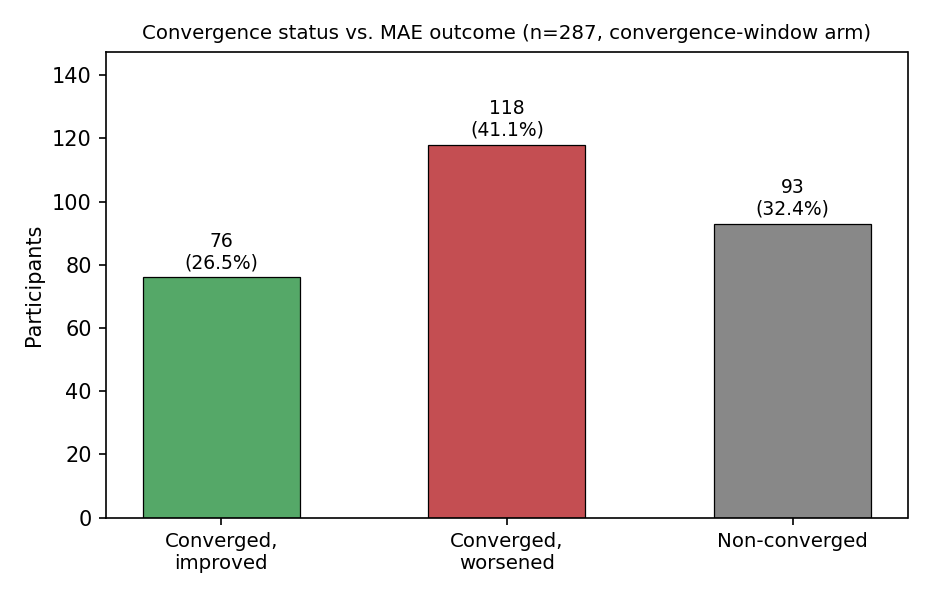
\includegraphics[width=0.66\linewidth]{figures/generated/personalization_convergence_outcome_crosstab.png}
\caption{Convergence status vs.\ MAE outcome under the convergence-based window (n=287).}
\label{fig:pers_conv_crosstab}
\end{figure}
